% =============================================================================
% 第三章原稿备份（基于 Lag 特征的集成学习方法研究）
% 自 body/graduate/content.tex 移出，供重写时查阅表格/图/实验数据。
% 备份日期：2026-06-09
% =============================================================================

\chapter{基于Lag特征的集成学习方法研究}

前两章详细阐述了 SSD 故障预测领域的研究现状与理论基础。围绕 SMART 等遥测数据的预测研究，既有工作在多视图时序特征、特征工程与模型组合等方面持续进展\cite{zhang2023multi,wang2022ssd}，低误报约束下的可部署预测亦是数据中心场景关注的热点\cite{chen2022ssd}；Xu 等人开源的大规模 SSD 数据集则为相关方法的训练与对比提供了公共基准\cite{xu2021general}。

本章在该数据集上选取 MB1 型号的 MLC-SSD，提出融合 Lag 特征、时间窗口统计特征与随机森林集成学习的预测流程：时序构造用于刻画 SMART 属性的动态演化，集成学习有助于在噪声与高维条件下获得较稳健的判别边界。
如图~\ref{fig:chap3-pipeline}所示，本文提出方法通过构建时序相关特征（Lag特征、时间窗口统计特征等）来捕捉SMART属性的动态变化模式，并采用随机森林集成学习模型进行故障预测。
实验结果表明，该方法在低误报率约束条件下能够取得较好的预测性能。

\begin{figure}[htbp]
    \centering
    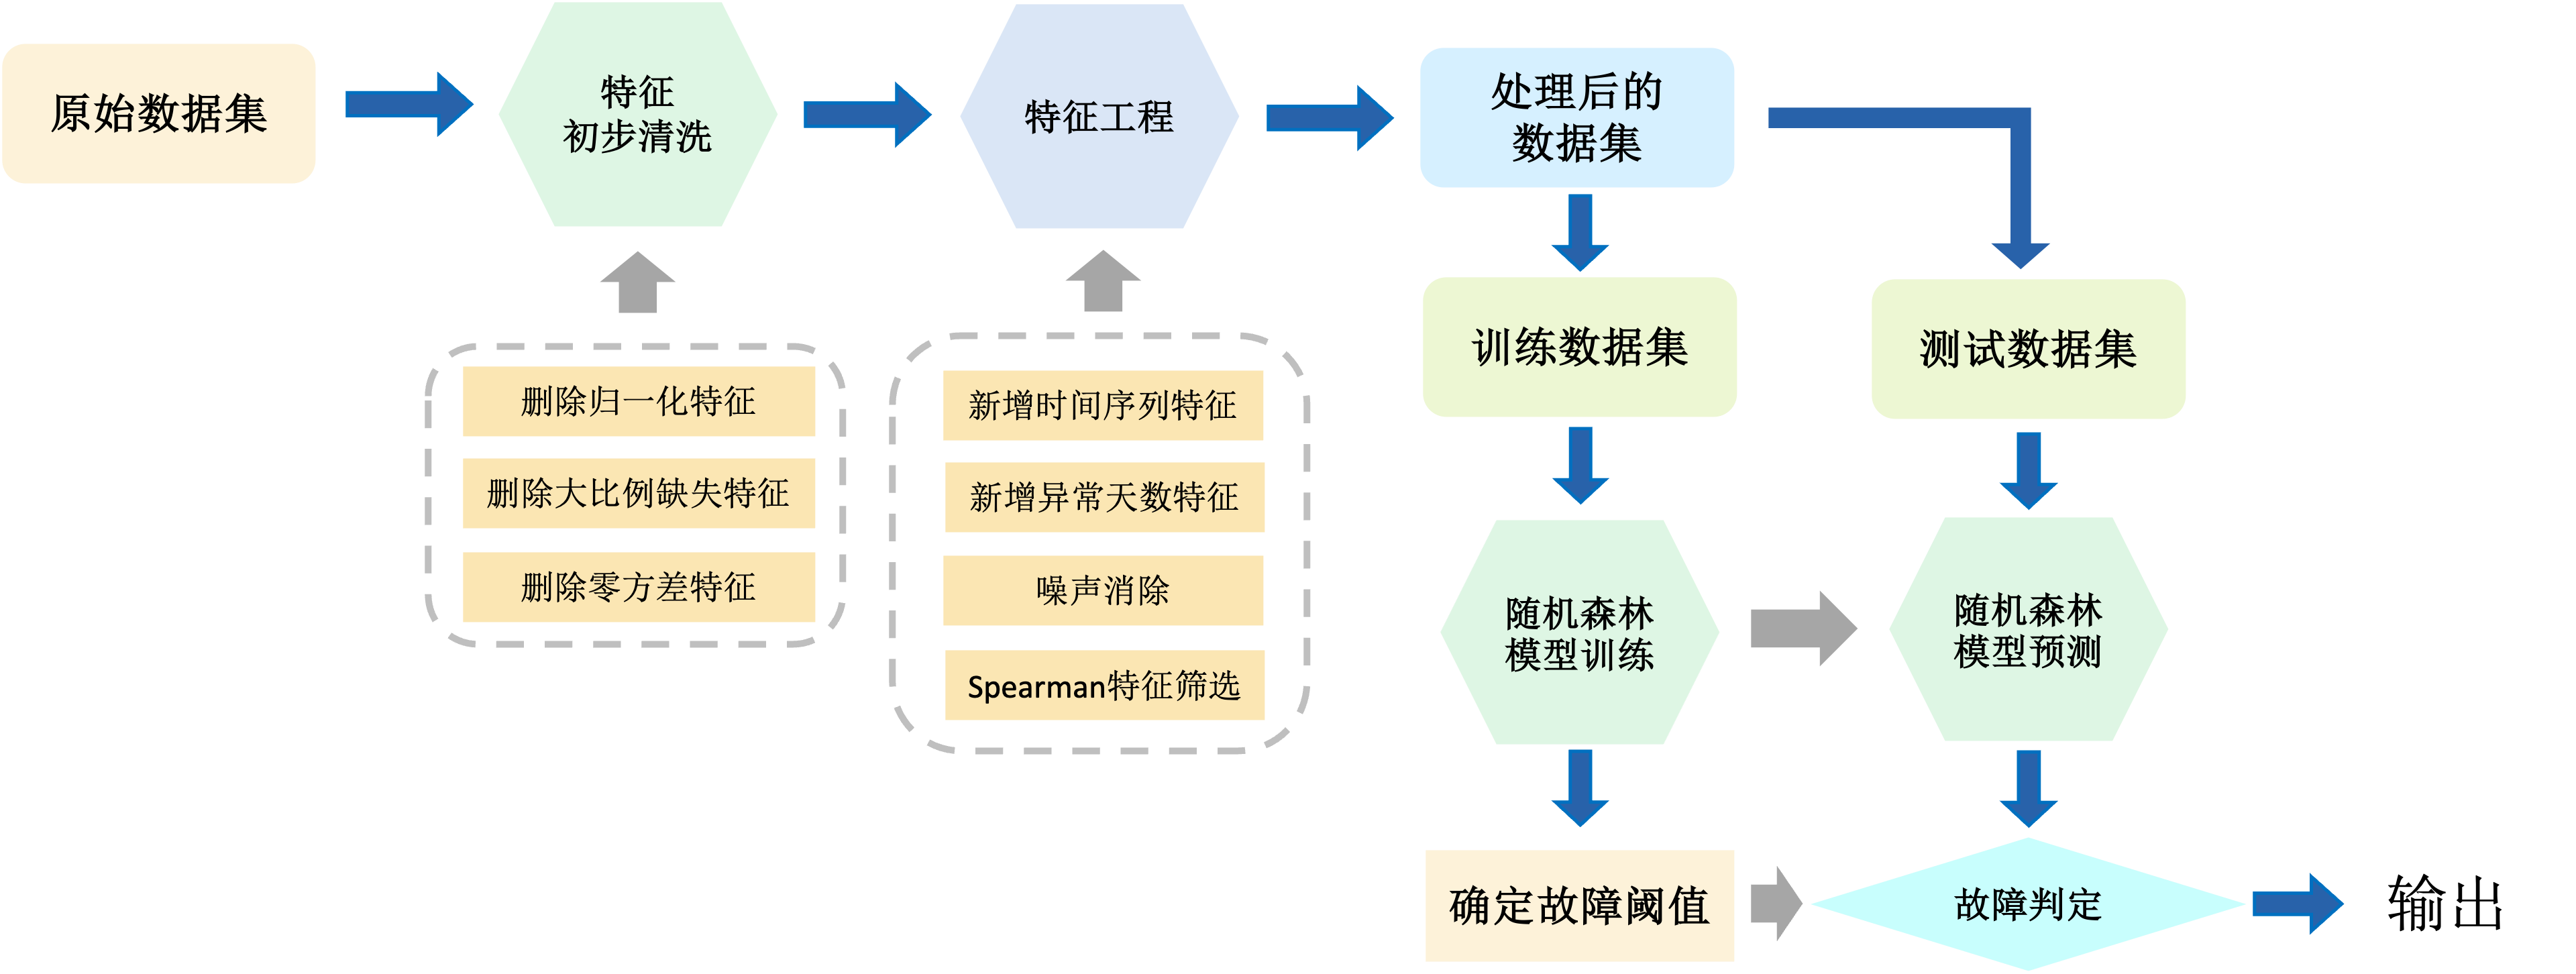
\includegraphics[width=0.92\linewidth]{figure/chap3-pipeline.png}
    \caption{第三章故障预测方法的数据流水线}
    \label{fig:chap3-pipeline}
\end{figure}

\section{数据集介绍与数据分析}

\subsection{数据集概述}

本研究采用的数据集来源于阿里云提供的大型SSD故障预测数据集\cite{xu2021general}。该数据集包含SSD盘每日SMART监控数据，时间跨度为2018年至2019年，数据规模达到千万级别。数据集涵盖了多种型号的SSD，本文主要针对数据集中的MB1型号的MLC-SSD进行分析和建模。

原始数据集中，每条样本包含102个特征维度，包括：
\begin{itemize}
    \item 原始SMART属性值
    \item 归一化后的SMART属性值
\end{itemize}

由于不同厂商对SMART属性的定义和归一化标准存在差异，原始数据集存在特征维度高、无效特征多、数据质量不一致等问题，需要进行系统的数据预处理和特征工程。

\subsection{数据集统计分析}

\subsubsection{数据规模统计}

MB1型号SSD数据集的基本统计信息如表\ref{tab:mb1-dataset-stats}所示。
\begin{table}[htbp]
    \centering
    \caption{\label{tab:mb1-dataset-stats}MB1型号SSD数据集基本统计信息}
    \begin{tabularx}{0.78\linewidth}{lX}
        \toprule
        统计项 & 数值说明 \\
        \midrule
        SSD总数 & 超过40,000块 \\
        总记录数 & 千万级别（约10,000,000条） \\
        时间跨度 & 2018年1月至2019年12月，共24个月 \\
        故障盘数量 & 约1400块（故障率约3.5\%） \\
        平均每块SSD记录数 & 约700条 \\
        \bottomrule
    \end{tabularx}
\end{table}

\subsubsection{故障特点分析}

从故障时间分布看，如图\ref{fig:failure-by-month}所示，除2018年5月出现明显峰值外，其余月份的故障磁盘数量整体较为均匀。

该结果说明故障并未集中在少数固定时间段，而是在较长观测周期内持续发生，具有一定随机性与长期累积特征。2018年5月的局部峰值可能与该阶段设备服役时长、负载波动或环境条件变化等因素叠加有关，但从全局趋势看，月度故障数量未呈现单调上升或单调下降。

\begin{figure}[htbp]
    \centering
    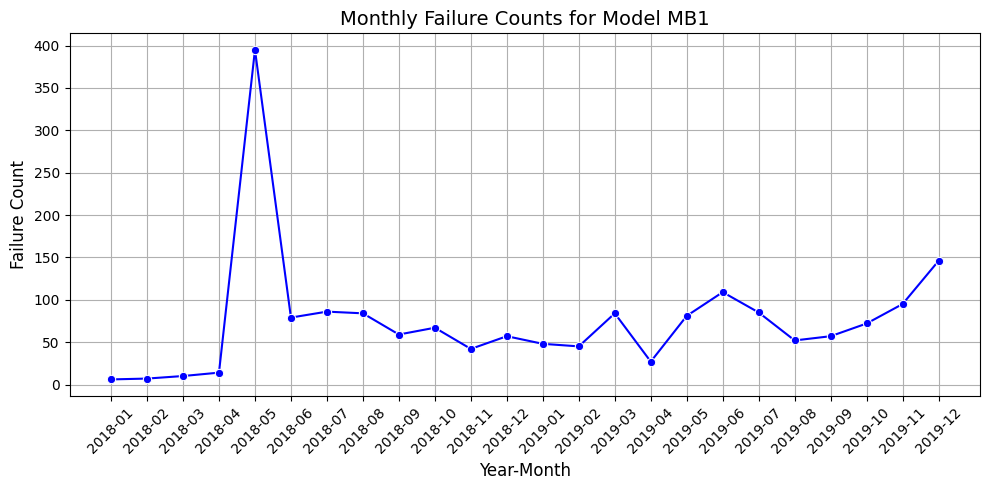
\includegraphics[width=0.9\linewidth]{figure/failure-by-month.png}
    \caption{MB1型号固态硬盘月度故障数量分布}
    \label{fig:failure-by-month}
\end{figure}


从故障演化特征看，如图\ref{fig:failure-disk-sample}所示，故障磁盘与健康磁盘在关键SMART属性上的时序轨迹存在明显差异。

\begin{figure}[htbp]
    \centering
    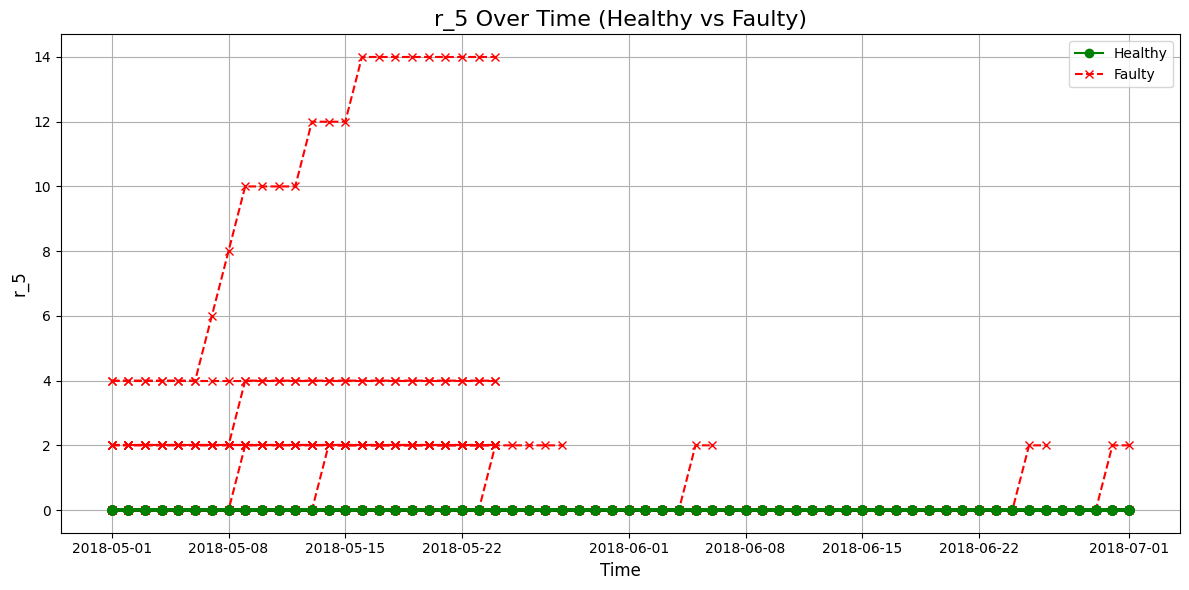
\includegraphics[width=0.82\linewidth]{figure/failure-disk-sample.png}
    \caption{故障磁盘样本的指标时序变化示意图}
    \label{fig:failure-disk-sample}
\end{figure}

以SMART属性重映射扇区计数r\_5为例，绿色曲线对应健康磁盘，在观测窗口内基本保持为0；红色曲线对应故障磁盘，在失效前会出现持续上升。该上升过程可视为故障前兆，且其持续时长存在显著差异，可由数天延续至数月。

\subsubsection{数据质量分析}

数据观察结果显示：各特征缺失值比例介于0\%至85\%，平均缺失率约70\%；部分特征存在空值描述不一致和离群值；所有磁盘均存在特定日期日志缺失，其中约83\%出现随机日期缺失或连续日志中断。因此，后续建模前需对缺失值、异常值和时序断点进行针对性处理。

\subsection{数据预处理}

\subsubsection{特征初步筛选}

针对原始数据集的特征冗余问题，采用以下策略进行初步特征筛选：

\begin{itemize}
    \item 删除大比例缺失特征：删除缺失值比例超过80\%的特征，这些特征信息量不足，对模型训练贡献有限
    \item 删除零方差特征：删除方差为0的特征，即所有样本取值相同的特征，这些特征无法提供区分信息
    \item 删除归一化特征：由于不同厂商的归一化标准不同，归一化特征的可用度和可比性较低，因此仅保留原始SMART属性值
\end{itemize}

经过初步筛选后，保留16个原始SMART特征，如表\ref{tab:smart-features}所示，覆盖磨损相关指标（如通电时间、LBA写入/读取总数）、错误计数指标（如重映射扇区计数、编程/擦写失败计数）以及温度相关指标。

\begin{table}[htbp]
    \caption{\label{tab:smart-features}初步筛选后保留的SMART特征}
    \begin{tabularx}{\linewidth}{cX<{\centering}X<{\centering}X<{\centering}}
        \toprule
        ID & 中文名称 & 英文名称 & 特征类型 \\
        \midrule
        5 & 重映射扇区计数 & \mbox{Reallocated Sectors Count} & 错误计数 \\
        9 & 通电时间累计 & Power-On Time Count & 磨损相关 \\
        12 & 通电周期计数 & Power Cycle Count & 磨损相关 \\
        177 & 磨损范围对比值 & Wear Range Delta & 磨损相关 \\
        180 & 未用的备用块计数 & Unused Reserved Block Count Total & 磨损相关 \\
        181 & 编程失败计数 & Program Fail Count & 错误计数 \\
        182 & 擦写失败计数 & Erase Fail Count & 错误计数 \\
        183 & 串口降速错误计数 & \mbox{SATA Downshift Error Count} & 错误计数 \\
        184 & 点到点错误检测计数 & End to End Error Detection Count & 错误计数 \\
        187 & 无法校正的错误 & \mbox{Reported Uncorrectable Errors} & 错误计数 \\
        190 & 气流温度 & Airflow Temperature & 环境指标 \\
        194 & 温度 & Temperature & 环境指标 \\
        195 & 编程错误块计数 & \mbox{Program Failure block Count} & 错误计数 \\
        199 & Ultra ATA 访问校验 \newline 错误率 & \mbox{Ultra ATA CRC Error Rate} & 错误计数 \\
        241 & LBA写入总数 & Total LBAs Written & 磨损相关 \\
        242 & LBA读取总数 & Total LBAs Read & 磨损相关 \\
        \bottomrule
    \end{tabularx}
\end{table}

\subsubsection{缺失值处理}

原始数据集中存在部分缺失值，可能由设备故障、网络中断或系统维护等原因导致，部分SSD的SMART日志甚至存在整日缺失。

为保持时间序列连续性，本文采用前向填充（Forward Fill）补全缺失值：优先使用该磁盘历史时刻最近有效观测值；对于序列起始位置等不存在前向有效值的情况，使用健康磁盘对应特征均值补充，以避免样本大量丢弃并降低噪声引入风险。

具体而言，对于特征$X$在时刻$t$的缺失值，填充方法如下：

\begin{itemize}
    \item 前向填充：$X_t = X_{t-1}$（如果$X_{t-1}$存在）
    \item 均值补充：$X_t = \mu_X^{\text{healthy}}$（如果不存在前向有效值，那么公式中的$\mu_X^{\text{healthy}}$表示所有健康样本在特征$X$上的均值）
\end{itemize}

本文认为该策略在保留时序连续性的同时，提高了缺失值处理的稳健性。

\subsection{故障标记策略}

SSD故障预测的目标是提前识别未来一段时间内可能发生故障的磁盘，以便运维人员及时采取预防措施。
在构建训练标签时，需要在预测提前量与标签准确性之间权衡，常见做法是将故障发生前一定时间窗口内的记录标记为正样本，其示意如图\ref{fig:label-strategy}所示：

\begin{figure}[htbp]
    \centering
    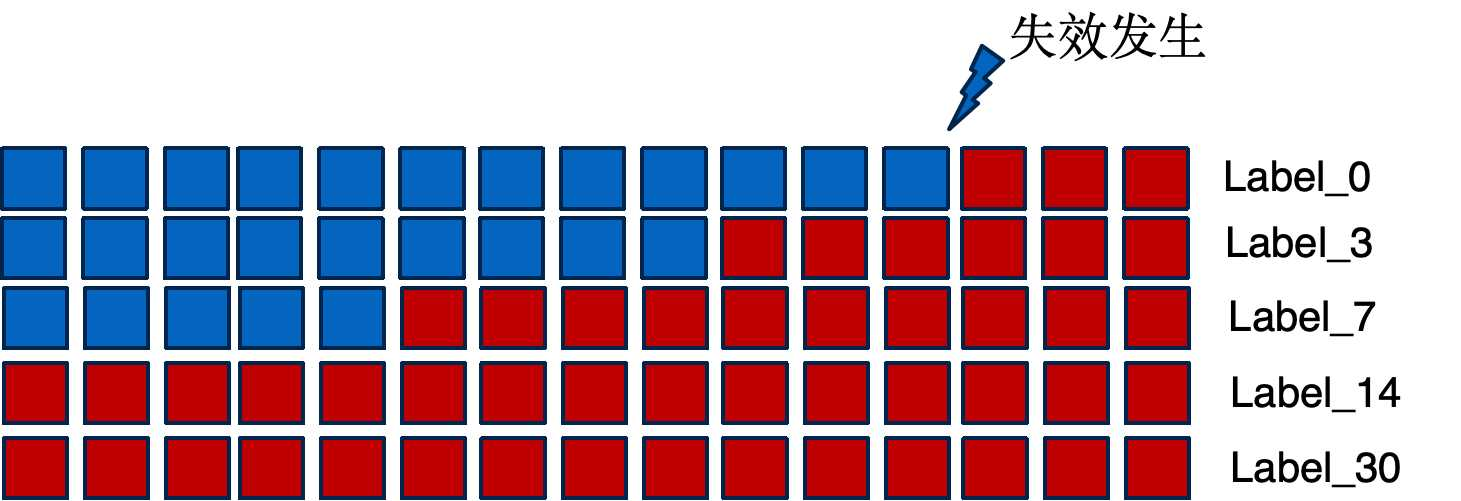
\includegraphics[width=0.72\linewidth]{figure/标签策略.jpg}
    \caption{故障标记时间窗口示意图}
    \label{fig:label-strategy}
\end{figure}

标签时间窗口并非越长越好或越短越好。图\ref{fig:label-strategy}给出了标记窗口的直观示意，其中蓝色方格表示负样本，红色方格表示正样本；在此基础上，表\ref{tab:label-strategies}进一步给出不同窗口策略的标注规则及其数学表示：

\begin{table}[htbp]
    \caption{\label{tab:label-strategies}故障标记策略}
    \begin{tabularx}{\linewidth}{cX<{\centering}X<{\centering}X<{\centering}}
        \toprule
        标记策略 & 定义 & 数学表示 \\
        \midrule
        label\_30 & 故障发生前30天及以后的记录标记为正样本 & $y_t = 1$ if $t \geq t_f - 30$ \\
        label\_14 & 故障发生前14天及以后的记录标记为正样本 & $y_t = 1$ if $t \geq t_f - 14$ \\
        label\_7 & 故障发生前7天及以后的记录标记为正样本 & $y_t = 1$ if $t \geq t_f - 7$ \\
        label\_3 & 故障发生前3天及以后的记录标记为正样本 & $y_t = 1$ if $t \geq t_f - 3$ \\
        label\_0 & 故障发生当天及以后的记录标记为正样本 & $y_t = 1$ if $t \geq t_f$ \\
        \bottomrule
    \end{tabularx}

    \vspace{2pt}
    \begin{minipage}{\linewidth}
        \footnotesize 注：$t_f$表示故障发生日期，$y_t$表示时刻$t$的标签（1表示正样本，0表示负样本）。
    \end{minipage}
\end{table}

结合表\ref{tab:label-strategies}中的各窗口定义可以看出，标签窗口长度会直接影响样本划分边界。
窗口过短时，模型难以充分捕捉故障前的渐进变化；窗口过长时，故障SSD在早期仍相对正常的样本可能被提前标记为故障，从而增加标签噪声并诱发过早预警。

此外，过长窗口还可能引入时间信息泄露风险。由于本文的任务目标是预测未来30天内可能发生故障的SSD，因此将最长标签窗口限定为30天，不采用超过30天的标记策略。
实验结果表明，label\_30 策略在保证预测性能的同时能够提供足够的预警时间，因此本文最终采用 label\_30 作为故障预测的标记策略。

\section{基于Lag特征的特征工程方法}

\subsection{时序特征构建的必要性}

由于SSD的故障是一个渐进的过程，SMART属性随时间的变化趋势包含了重要的健康信息\cite{chakraborttii2023leveraging}，故障发生前SMART属性会出现异常变化趋势。仅使用单点时刻的特征值难以捕捉这种动态变化模式。因此，构建时序相关特征对于提升故障预测性能至关重要。

传统的特征工程方法主要关注特征的静态统计特性，而忽略了时间维度上的信息。参考Xu等人的研究\cite{xu2021general}，本研究提出构建Lag特征和时间窗口统计特征，以捕捉SMART属性的时序变化模式。

\subsection{Lag特征构建}

Lag特征（滞后特征）是时间序列分析中的经典特征工程方法，通过引入历史时刻的特征值来捕捉时序依赖关系。对于SSD故障预测任务，Lag特征能够反映SMART属性的变化趋势，有助于识别故障前的异常模式。

对于每个SMART特征$X$，构建1至$k$天的Lag特征，即：
\begin{equation}
    X_{t-\text{lag}} = \{X_{t-1}, X_{t-2}, \ldots, X_{t-k}\},
\end{equation}
公式中的$X_t$表示当前时刻$t$的特征值，$\text{lag} \in \{1, 2, \ldots, k\}$表示滞后期数。本研究设置$k=7$，即构建1至7天的Lag特征。

Lag特征的构建基于以下假设：故障发生前的异常变化往往具有持续性，通过观察历史时刻的特征值，可以更好地识别这种异常趋势。

\subsection{时间窗口统计特征}

除 Lag 特征外，本文进一步构建滑动时间窗口统计特征，以刻画 SMART 属性在局部时间段内的变化模式。针对特征$X$，各统计量定义见表\ref{tab:window-stat-features}：
\begin{table}[htbp]
    \caption{\label{tab:window-stat-features}滑动时间窗口统计特征定义}
    \begin{tabularx}{\linewidth}{>{\centering\arraybackslash}m{1.6cm} >{\centering\arraybackslash}X >{\raggedright\arraybackslash}m{4.8cm}}
        \toprule
        统计量 & 数学定义 & 作用解释 \\
        \midrule
        最小值 & $\min(X_{t-w:t}) = \min\{X_{t-w}, X_{t-w+1}, \ldots, X_t\}$ & 反映特征值下界，异常样本常出现下界偏移。 \\
        最大值 & $\max(X_{t-w:t}) = \max\{X_{t-w}, X_{t-w+1}, \ldots, X_t\}$ & 反映特征值上界，异常样本常出现上界抬升。 \\
        平均值 & $\text{mean}(X_{t-w:t}) = \frac{1}{w+1}\sum_{i=t-w}^{t} X_i$ & 反映特征值整体水平，故障前可能出现均值漂移。 \\
        极差 & $\text{range}(X_{t-w:t}) = \max(X_{t-w:t}) - \min(X_{t-w:t})$ & 反映窗口内波动幅度，故障前可能出现波动加剧。 \\
        差分 & $\text{diff}(X_t) = X_t - X_{t-1}$ & 反映短期变化速度，故障前可能出现突发变化。 \\
        \bottomrule
    \end{tabularx}

    \vspace{2pt}
    \begin{minipage}{\linewidth}
        \footnotesize 注：$w$表示时间窗口大小，本文设定$w=7$，即使用过去7天数据进行统计计算。
    \end{minipage}
\end{table}

上述统计特征与 Lag 特征形成互补：Lag 特征反映相邻时刻的局部变化，窗口统计特征则提供区间尺度上的整体刻画，从而为后续模型学习提供更稳定的输入表示。进一步地，不同统计量对异常演化的敏感性存在差异，联合建模可同时覆盖“缓慢漂移”与“突发波动”两类退化模式，提升低误报约束下的可分性。

\subsection{基于Spearman相关系数的特征筛选}

经过特征工程后，特征维度显著增加。假设原始特征数为$d$，Lag特征数为$k$，统计特征数为$s$，则总特征数可达到$d \times (k + s)$，特征维度可能达到数百甚至上千维。为降低模型复杂度、减少过拟合风险，需要进行特征筛选。

本研究采用Spearman相关系数进行特征筛选。Spearman相关系数是一种非参数统计方法，能够衡量两个变量之间的单调关系。对于特征$X$和目标变量$Y$，Spearman相关系数定义为：

\begin{equation}
    \label{equ:spearman}
    \rho_s = 1 - \frac{6\sum_{i=1}^{n} d_i^2}{n(n^2-1)},
\end{equation}
公式中的$d_i$表示$X$和$Y$的秩次差，$n$表示样本数。Spearman相关系数的取值范围为$[-1, 1]$，绝对值越大表示相关性越强。

相比Pearson相关系数，Spearman相关系数具有以下优势：
\begin{itemize}
    \item 非参数性：不要求数据服从正态分布
    \item 对异常值鲁棒：基于秩次计算，对异常值不敏感
    \item 捕捉非线性关系：能够识别单调的非线性关系
\end{itemize}

通过计算每个特征与目标变量（故障标签）的Spearman相关系数，按绝对值大小排序，筛选出Top $m$个与故障最相关的特征作为最终训练特征。本研究设置$m=80$。实验结果表明，特征筛选能够在保持预测性能的同时，显著降低模型复杂度。

\subsection{基于故障机理的噪声样本移除}

从SSD故障的物理机理出发，故障可概括为两类。第一类是由长期使用引起的自然老化失效，常见表现包括寿命到期和预留空间耗尽。第二类是由硬件缺陷或环境扰动触发的突发异常故障，典型现象包括控制器损坏和NAND闪存错误。两类故障在形成过程和演化速度上存在明显差异，因此在SMART属性上的响应模式也不相同。

基于上述差异，本文将SMART特征划分为磨损相关组A和突发异常组B。A组用于刻画长期磨损状态，主要包含通电时间、通电周期以及LBA写入总量与读取总量，对应特征9、特征12、特征241和特征242。B组用于表征短期异常信号，主要由多类错误计数构成，包括特征5、特征181、特征182、特征187和特征195。对健康硬盘而言，B组中的多数指标长期保持在零附近，只有在故障临近或异常突发时才会出现明显跃迁。对于故障盘$i$，记$A_i$和$B_i$分别为其在A组和B组上的特征值。

由此可见，能够被模型稳定识别的故障样本通常同时呈现一定的磨损累积与异常信号抬升；相反，若样本仅表现为磨损增强而缺乏异常跃迁，则更可能落入健康样本分布附近，形成训练噪声。基于这一判别思路，构建如下噪声样本识别规则：如果故障盘$i$满足以下条件，则视为噪声样本：
\begin{equation}
    B_i < \theta_B \text{ 且 } A_i > \theta_A,
\end{equation}
公式中的$\theta_A$和$\theta_B$分别为磨损特征和突发异常特征的阈值。这类故障盘仅表现出磨损特征的增加，而没有任何突发异常特征的变化，与正常磨损的健康盘在特征空间上难以区分，容易导致模型学习到错误的模式。

为直观说明该类样本的可分性问题，抽取部分磁盘样本的相关属性进行可视化，如图\ref{fig:mutation-feature-noise}所示：
\begin{figure}[htbp]
    \centering
    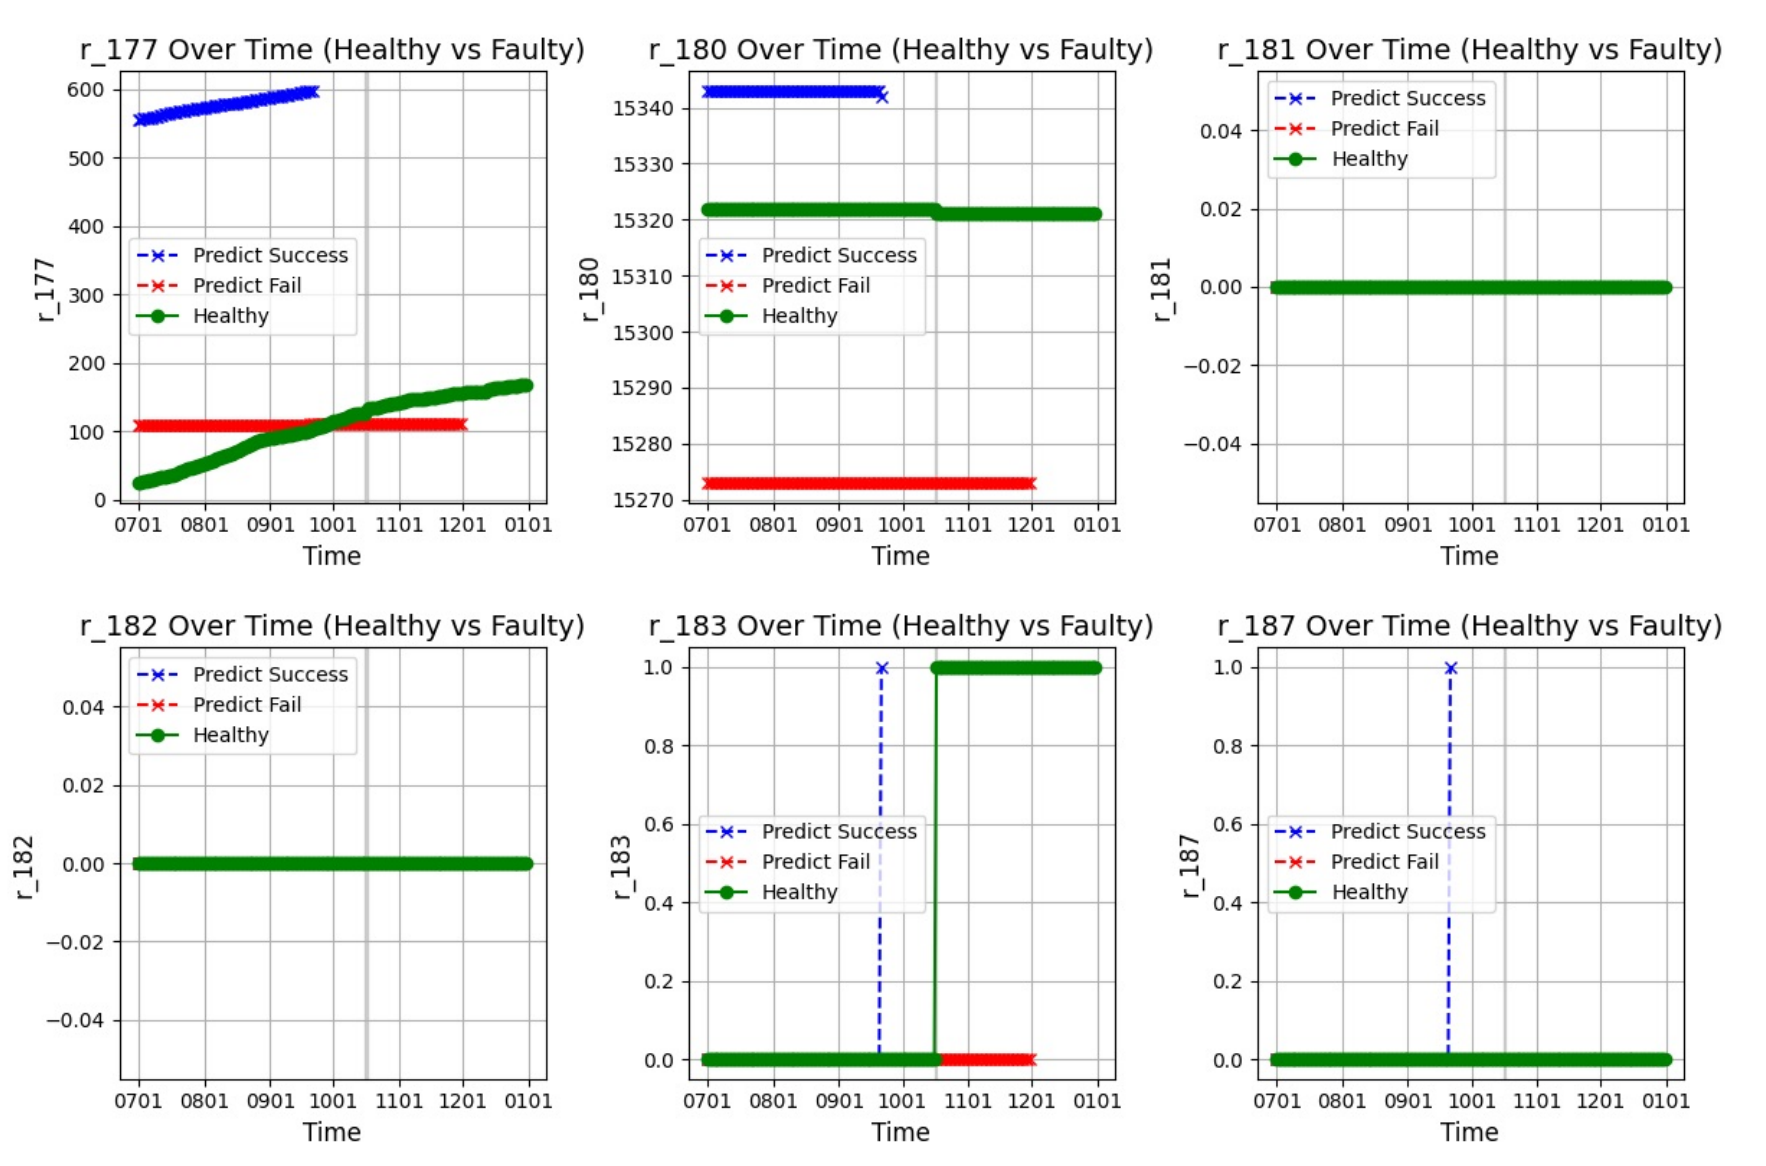
\includegraphics[width=0.72\linewidth]{figure/突变特征.png}
    \caption{突变特征与噪声样本变化趋势示意图}
    \label{fig:mutation-feature-noise}
\end{figure}

图中红色曲线表示噪声硬盘样本的变化趋势，绿色曲线表示健康硬盘样本的变化趋势，蓝色曲线表示可被模型识别出的故障样本突变趋势，典型对应特征183和特征187。
在缺乏额外信息的情况下，噪声样本在各属性维度上的变化轨迹与健康样本高度重合，图中常表现为仅能观察到绿色直线，因此这类样本难以与健康样本有效区分。将该类样本从训练集中移除，能够提升模型对真实异常信号的识别能力。

\section{实验结果与分析}

\subsection{实验设置}

\subsubsection{数据集划分} 

采用按时间顺序的划分方式进行数据集划分，具体如下：
\begin{itemize}
    \item 训练集：2018年1月至2019年7月的数据（共计19个月）
    \item 测试集：2019年9月至2019年11月的数据（共计3个月）
\end{itemize}
这种划分方式是为了符合实际应用场景，即使用历史数据训练模型，预测未来数据。
需要说明的是，为避免训练与测试窗口之间的时间重叠带来数据泄露风险，训练集在 2019 年 7 月结束，不包含 2019 年 8 月的数据。
测试区间选择2019年9月至11月而不包含12月，主要是因为12月数据位于观测期末端，数据集中没有2020年1月的故障清单，会因为故障标签不完整导致评估失真。

\subsubsection{评估指标}

盘级故障预测效果的评估流程参考了数据算法赛 PAKDD2020 阿里巴巴智能运维算法大赛所公开的评测设定\cite{he2020large}。
在此基础上，本研究采用盘级评估方式，即对于每块SSD，在评估窗口内若存在预测为故障的记录，则取最早一次预测为故障的日期，并判断该日期后30天内SSD是否实际发生故障，具体的判定规则如图~\ref{fig:tp-fp-tn-fn}所示：
\begin{figure}[htbp]
    \centering
    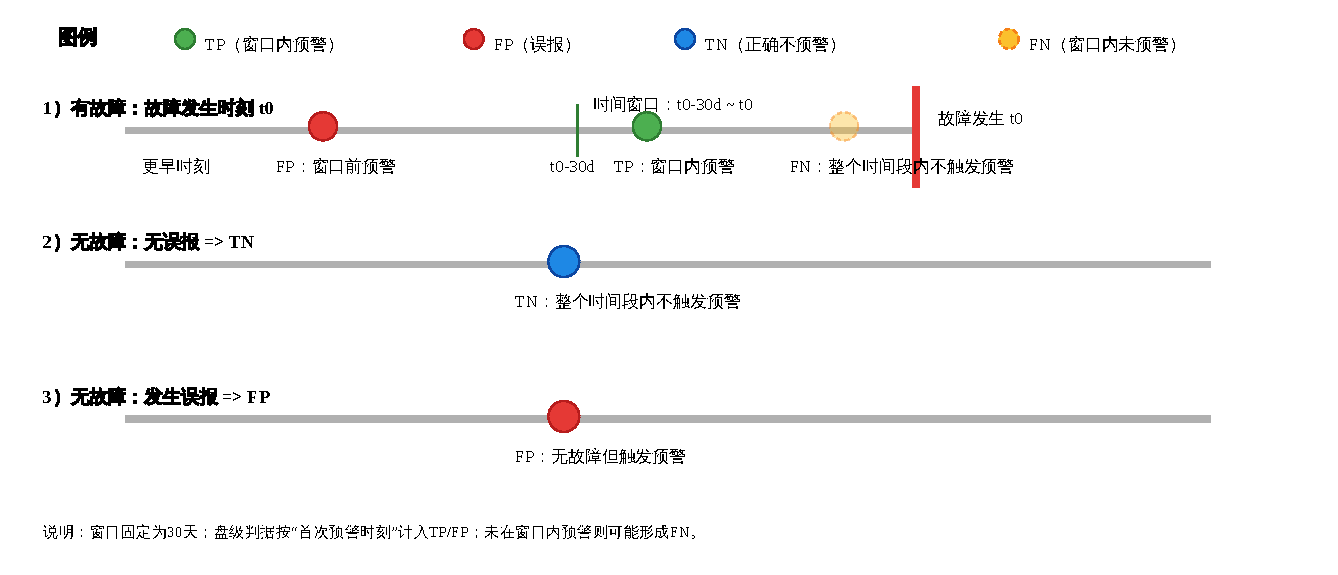
\includegraphics[width=0.90\linewidth]{figure/tp_tn_fp_fn.pdf}
    \caption{盘级评估中 TP/FP/TN/FN 判定规则示意图}
    \label{fig:tp-fp-tn-fn}
\end{figure}

基于上述判定规则得到的混淆矩阵，定义以下评估指标：
\begin{itemize}
    \item 真正例率：$TPR = \frac{TP}{TP+FN}$，表示实际故障盘中被正确预测的比例，也称为召回率（Recall；对应图中时间窗口内的命中判定）
    \item 假正例率：$FPR = \frac{FP}{FP+TN}$，表示正常盘中被错误预测为故障的比例（对应图中的误报判定）
\end{itemize}

在实际应用中，FPR过高会导致运维成本增加，因此需要在控制FPR的前提下最大化TPR。本研究设定FPR约束条件为$\leq 0.035\%$，通过调整分类阈值来满足该约束。

\subsubsection{实验配置}

实验采用随机森林作为基础模型，主要考虑以下因素：
\begin{itemize}
    \item 抗噪声能力：随机森林通过随机子采样和特征选择能够降低对噪声的敏感度
    \item 处理数据不平衡：通过调整样本权重能够有效应对故障样本稀少的问题
    \item 特征重要性分析：能够提供特征重要性度量，便于后续分析和解释
\end{itemize}

随机森林的主要超参数设置如表\ref{tab:rf-hyperparams}所示。

\begin{table}[htbp]
    \centering
    \caption{\label{tab:rf-hyperparams}随机森林主要超参数设置}
    \begin{tabularx}{\linewidth}{>{\raggedright\arraybackslash}X >{\centering\arraybackslash}X}
        \toprule
        参数名称 & 设置值 \\
        \midrule
        树的数量（n\_estimators） & 100 \\
        最大深度（max\_depth） & 20 \\
        最小样本分裂数（min\_samples\_split） & 5 \\
        最小样本叶子数（min\_samples\_leaf） & 2 \\
        特征子集大小（max\_features） & $\sqrt{d}$（公式中的$d$为特征数） \\
        \bottomrule
    \end{tabularx}
\end{table}

\subsection{整体实验结果}

在FPR $\leq 0.035\%$的统一约束下，本文方法在MB1型号SSD数据集上表现稳定。下文将从特征工程、标记策略、特征筛选与噪声样本处理四个方面展开分项分析，并在对应表格中给出具体指标结果。

\subsection{特征工程效果分析}

为验证特征工程的有效性并分析各类特征的贡献，本文在随机森林模型与 FPR $\leq 0.035\%$ 的统一约束下，对不同特征组合进行对比实验，并从检出率提升与误报控制两个维度评估其效果，结果如表\ref{tab:feature-engineering}所示：

\begin{table}[htbp]
    \centering
    \caption{\label{tab:feature-engineering}不同特征组合下的预测性能对比}
    \begin{tabular*}{0.88\linewidth}{@{\extracolsep{\fill}}ccccc@{}}
        \toprule
        Lag特征 & 统计特征 & 原始特征 & TPR & FPR \\
        \midrule
        & & $\bullet$ & 4.46\% & $\leq 0.035\%$ \\
        $\bullet$ & & & 33.48\% & $\leq 0.035\%$ \\
        & $\bullet$ & & 32.30\% & $\leq 0.035\%$ \\
        $\bullet$ & $\bullet$ & & 39.21\% & $\leq 0.035\%$ \\
        $\bullet$ & $\bullet$ & $\bullet$ & 39.65\% & $\leq 0.035\%$ \\
        \bottomrule
    \end{tabular*}
    
    \vspace{2pt}
    \begin{minipage}{0.88\linewidth}
        \footnotesize 注：Lag、统计、原始三列中，实心圆点（$\bullet$）表示该类型特征参与建模，空白表示不纳入。
    \end{minipage}
\end{table}

由表\ref{tab:feature-engineering}可知，仅使用 16 维原始 SMART 属性时 TPR 仅为 4.46\%；单独引入 Lag 特征或时间窗口统计特征时，TPR 分别升至 33.48\% 与 32.30\%，说明相对单点原始读数，时序构造特征能更有效地反映故障前兆。将两类构造特征联用后（约 200+ 维），TPR 达到 39.21\%，相对基线提升约 7.8 倍；再并入当前时刻的原始属性列后，TPR 进一步提高至 39.65\%。Lag 特征引入历史轨迹，时间窗口统计量刻画区间内的边界与波动强度，二者与原始属性互补，有助于同时捕捉渐进退化与短期异常。

\subsection{不同标记策略对比}

不同标记策略的对比结果表明，在 FPR 均满足 $\leq 0.035\%$ 的前提下，TPR 随预警窗口变化并不呈简单单调关系：3 天与 14 天窗口均为 39.21\%，7 天窗口略降至 38.33\%，可视为标记边界与样本划分带来的正常波动，整体仍处在同一性能水平。
在此范围内，label\_30 同时达到最高 TPR 与最长预警时间，即在误报可控条件下兼顾检出能力与运维提前量，故本文最终采用 label\_30 作为标记策略。具体结果见表\ref{tab:label-comparison}：

\begin{table}[htbp]
    \centering
    \caption{\label{tab:label-comparison}不同标记策略性能对比}
    \begin{tabularx}{0.88\linewidth}{>{\raggedright\arraybackslash}X >{\centering\arraybackslash}X >{\centering\arraybackslash}X >{\centering\arraybackslash}X}
        \toprule
        标记策略 & TPR & FPR & 预警时间 \\
        \midrule
        label\_0 & - & - & 0天 \\
        label\_3 &  39.21\% & $\leq 0.035\%$ & 3天 \\
        label\_7 &  38.33\% & $\leq 0.035\%$ & 7天 \\
        label\_14 & 39.21\% & $\leq 0.035\%$ & 14天 \\
        label\_30 & 39.65\% & $\leq 0.035\%$ & 30天 \\
        \bottomrule
    \end{tabularx}
\end{table}

\subsection{特征筛选效果分析}

不同特征维度设置下的性能与运行时间对比如表\ref{tab:spearman-topk-comparison}所示。表格中的Top-$k$表示按Spearman相关性对特征进行排序后，保留相关性最高的前$k$个特征用于训练。

\begin{table}[htbp]
    \centering
    \caption{\label{tab:spearman-topk-comparison}Spearman降维不同Top-$k$设置对比}
    \begin{tabularx}{0.72\linewidth}{>{\raggedright\arraybackslash}X >{\centering\arraybackslash}X >{\centering\arraybackslash}X}
        \toprule
        降维方式 & TPR & 运行时间 \\
        \midrule
        Top40 & 37.78\% & 223s \\
        Top70 & 40.09\% & 235s \\
        Top80 & 41.15\% & 295s \\
        Top90 & 40.97\% & 336s \\
        Top120 & 40.53\% & 384s \\
        Top160 & 39.65\% & 418s \\
        Top208 & 39.65\% & 459s \\
        \bottomrule
    \end{tabularx}
\end{table}

从表\ref{tab:spearman-topk-comparison}可以看出，在特征筛选中，随着$k$由大到小，TPR呈现先上升后下降的趋势：
当$k$由208逐步减小至80时，TPR由39.65\%提升至41.15\%；继续减小至40后，TPR下降至37.78\%。
这验证了过多特征会引入冗余信息并干扰模型训练，而特征数量过少又会导致模型表征能力不足。
与此同时，运行时间随$k$增大由223s上升至459s，呈现明显增长趋势。综合预测性能与计算成本，Top80在本实验设置下取得了较优平衡，因此后续实验采用该设置。
对筛选出的特征进行重要性分析，发现：
\begin{itemize}
    \item Lag特征在Top特征中占据重要地位，特别是Lag\_1和Lag\_2特征
    \item 统计特征中的mean和range特征重要性较高
    \item 原始特征中的错误计数类特征重要性较高，如重映射扇区计数（特征5）、无法校正错误（特征187）和编程错误块计数（特征195）；这些特征均与坏块计数相关，结果与工程直觉一致。
\end{itemize}

\subsection{噪声样本移除效果分析}

噪声样本移除前后性能对比如表\ref{tab:noise-removal}所示。移除噪声样本后，TPR从41.15\%提升至41.23\%，说明基于故障机理的噪声样本移除策略能够提升模型对真实异常信号的识别能力。

\begin{table}[htbp]
    \centering
    \caption{\label{tab:noise-removal}噪声样本移除前后性能对比}
    \begin{tabularx}{0.72\linewidth}{>{\raggedright\arraybackslash}X >{\centering\arraybackslash}X >{\centering\arraybackslash}X}
        \toprule
        噪声样本处理 & TPR & FPR \\
        \midrule
        保留噪声样本 & 41.15\% & $\leq 0.035\%$ \\
        移除噪声样本 & 41.23\% & $\leq 0.035\%$ \\
        \bottomrule
    \end{tabularx}
\end{table}

实验结果表明，移除噪声样本后，在FPR保持不变（$\leq 0.035\%$）的条件下，TPR由41.15\%提升至41.23\%，验证了移除噪声样本策略能够使模型更好地学习故障模式。

\subsection{不同学习模型对比}

为验证随机森林模型的选择合理性，对比了多种机器学习模型的性能，结果如表\ref{tab:model-comparison}所示。

对比对象涵盖不同方法范式：
单树模型决策树，树集成模型随机森林、XGBoost 和 LightGBM，无监督异常检测模型孤立森林，神经网络模型 MLP，以及时序建模模型 PatchTST 和 MVTRF；
PatchTST 采用分块建模思想：先将输入时间序列划分为长度固定的局部片段（patch），再以片段为粒度进行表示学习与依赖建模\cite{huang2024long}；MVTRF 采用多视图随机森林框架，将包含 Lag 信息的时序特征与统计分布特征联合建模，通过多视角特征学习提升故障识别能力\cite{zhang2023multi}。
为保证结论可比性，所有模型均在相同数据划分与一致的 FPR 约束下进行评估。

\begin{table}[htbp]
    \centering
    \caption{\label{tab:model-comparison}不同学习模型性能对比}
    \begin{tabularx}{0.72\linewidth}{>{\raggedright\arraybackslash}X >{\centering\arraybackslash}X >{\centering\arraybackslash}X}
        \toprule
        模型 & TPR & FPR \\
        \midrule
        随机森林 & 41.23\% & $\leq 0.035\%$ \\
        XGBoost & 40.27\% & $\leq 0.035\%$ \\
        LightGBM & 40.00\% & $\leq 0.035\%$ \\
        MVTRF & 40.47\% & $\leq 0.035\%$ \\
        决策树 & - & $> 0.035\%$ \\
        孤立森林 & 19.64\% & $\leq 0.035\%$ \\
        MLP & 33.63\% & $\leq 0.035\%$ \\
        PatchTST & 31.29\% & $\leq 0.035\%$ \\
        \bottomrule
    \end{tabularx}
    
    \vspace{2pt}
    \begin{minipage}{0.72\linewidth}
        \footnotesize 注：TPR 为“-”表示该模型在调参后仍无法满足 FPR 约束（$>0.035\%$），因此不报告对应 TPR。
    \end{minipage}
\end{table}

实验结果表明，随机森林在满足 FPR 约束的前提下取得最高 TPR，整体表现最优。
XGBoost 和 LightGBM 虽同属集成学习，但在当前噪声条件下略低于随机森林，可能是由于 Boosting 对噪声与弱表征正样本更敏感；
MVTRF 的 TPR 为 40.47\%，高于 XGBoost 和 LightGBM，说明融合时序与统计多视图特征（其中包含 Lag 信息）对提升检出能力具有积极作用；但其仍略低于本文随机森林方案，可能与当前任务以单一低 FPR 目标优化为主、样本规模有限且类别不平衡有关，多视图与多任务耦合带来的额外建模复杂度未能在该设定下充分转化为增益；
决策树在当前数据规模与噪声条件下易产生过拟合，导致其对局部异常模式过度敏感，调参后仍难以将 FPR 控制在约束范围内；
孤立森林因无法利用监督标签而表现较弱，MLP 在该表格型数据场景下也未达到树模型效果；
PatchTST 虽具备长序列建模能力，但本任务以结构化 SMART 特征与中短期退化信号为主，且样本噪声与类别不平衡较明显，在低 FPR 约束下其优势未能充分体现；
随机森林在本任务中兼顾了稳健性与预测性能，具有更好的适用性。

\subsection{误报与检出的权衡}

前文各表均在 FPR  $\leq 0.035\%$ 约束下报告 TPR，以便与运维可接受的误报水平对齐。为刻画误报约束放松时检出率如何变化，在相同的随机森林模型、特征工程与噪声样本处理流程下，通过调整分类器输出阈值，对测试集进行扫描，得到 FPR 与 TPR 的对应关系。
扫描结果如图~\ref{fig:fpr-tpr-tradeoff}所示：
\begin{figure}[htbp]
    \centering
    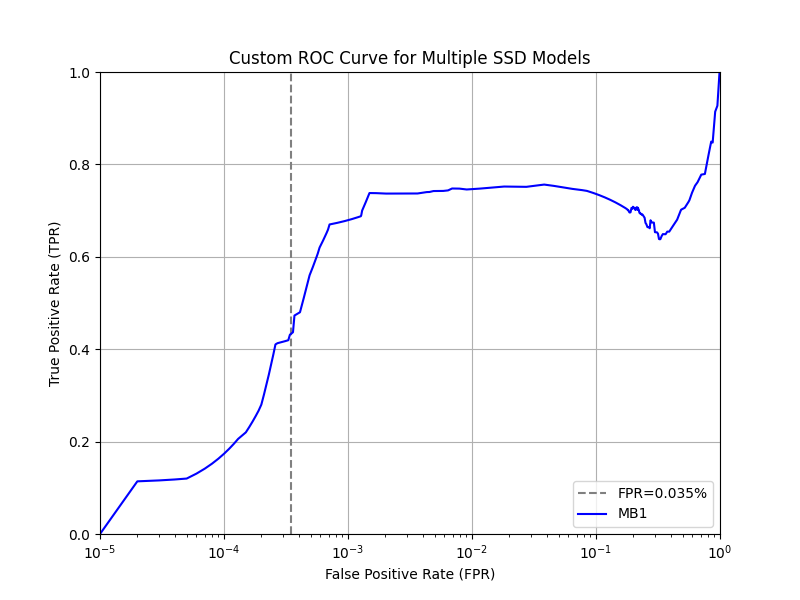
\includegraphics[width=0.7\linewidth]{figure/roc.png}
    \caption{调整分类阈值时盘级ROC曲线}
    \label{fig:fpr-tpr-tradeoff}
\end{figure}

需要说明的是，该曲线不等同于经典二分类问题中、在固定 0/1 样本标签下得到的 ROC 曲线。后者在理论上有随阈值扫描而单调变化的性质；而本文在盘级评估中引入了时间意义上的判据——若某块盘在距离真实故障仍较远的时间点即被首次判为阳性，则该次预警在业务上视为过早告警：在本文采用的统计口径中，将其计入假正例，而不将其视为对故障盘的正确检出并折算进 TPR。

在上述口径下，阈值从严到宽扫描时，TPR首先上升：模型会优先命中故障征兆更明显、相对容易识别的故障盘，正确检出数量随之增加。
随后模型进入更容易触发过早告警的区间，此时虽然 FPR 持续上升，但盘级 TPR 会阶段性下降。
当阈值继续放宽到能够在合理时间窗内覆盖更多真实故障盘时，TPR 会重新走高。需要注意的是，在本文盘级统计口径下，随着阈值放宽，部分原本计入 FN 的样本会转化为 TP，而部分过早告警样本会转化为 FP；因此在若干阈值区间内，TPR 计算式中的分子 TP 与分母（TP+FN）会同步变化，分母中 FN 占比下降，整体比值呈现向 $TP/TP$ 靠近的趋势，从而表现为 TPR 再次上升。这也是该评估口径在阈值扫描分析中的局限之一。

\subsection{方法局限性讨论}

本研究提出的方法虽然取得了较好的预测性能，但仍存在一定局限性。
首先，当前方法主要针对MB1型号的MLC-SSD进行优化，对于其他型号或类型的SSD，可能需要重新调整特征工程策略和模型参数，因为不同型号在SMART属性定义和故障模式上可能存在差异。
其次，标记策略的选择依赖于对故障前兆时间的先验知识，在实际应用中需根据具体场景动态调整，不同故障类型对应的最优标记策略也可能不同。
此外，Lag特征与时间窗口统计特征的构建增加了特征工程复杂度，对数据时序连续性提出了更高要求，在缺失较严重时往往需要额外的补全与稳健处理。与此同时，基于故障机理的噪声样本移除依赖先验故障类型划分，对于混合故障场景可能存在识别偏差，如何提升噪声样本识别准确性仍是后续工作重点。最后，虽然随机森林能够提供特征重要性，但对单次预测结果的细粒度解释能力仍有限，如何进一步提升模型可解释性、增强运维决策支持能力，仍有待深入研究。

\section{本章小结}

本章提出了一种基于Lag特征和集成学习的SSD故障预测方法。与仅追求检出率提升的方案不同，本文以低误报约束为核心设计目标，在保证FPR $\leq 0.035\%$的前提下系统优化模型检出能力。主要贡献包括：

\begin{enumerate}
    \item 提出了基于Lag特征的特征工程方法：通过构建1-7天的Lag特征和时间窗口统计特征，有效捕捉SMART属性的时序变化模式，将TPR从4.46\%提升至39.21\%，提升了约7.8倍。
    
    \item 设计了灵活的故障标记策略：通过对比不同标记策略，选择label\_30策略在保证预测性能的同时提供足够的预警时间。
    
    \item 提出了基于故障机理的噪声样本移除方法：通过区分磨损相关特征和突发异常特征，识别并移除难以区分的噪声样本，提升模型性能。
    
    \item 验证了随机森林在SSD故障预测任务上的有效性：通过对比多种机器学习模型，验证了随机森林在抗噪声和处理数据不平衡方面的优势。
    
    \item 进行了特征组合对比与特征重要性分析：在统一实验设置下汇总基线与多种特征组合的 TPR ，并结合 Top 特征的重要性排序说明各类构造的作用。
\end{enumerate}

实验结果表明，该方法在FPR $\leq 0.035\%$的严格约束下，能够达到41.23\%的TPR，说明本文方法在误报可控前提下实现了有效检出，为SSD故障预测提供了兼顾可靠性与实用性的解决方案。
该方法在实际应用中能够帮助运维人员提前识别潜在的故障风险，降低数据丢失风险，提升系统可靠性。
